\documentclass[12pt]{article}
\usepackage[a4paper,margin=0.75in]{geometry}
\usepackage[utf8]{inputenc}
\usepackage[OT1]{fontenc}
\usepackage[table,usenames,dvipsnames]{xcolor}
\usepackage{array}
\usepackage{varwidth}
\usepackage{tabularx}
\usepackage{amsmath}
\usepackage{hyperref}
\usepackage{enumitem}
\usepackage{graphicx}
\usepackage{tcolorbox}
\usepackage{forest}
\usepackage{parskip}
\renewcommand*\familydefault{\sfdefault}

\newtcolorbox{mybox}[3][]
{
  colframe = #2!25,
  colback  = #2!10,
  coltitle = #2!20!black,  
  title    = {#3},
  #1,
}

\hypersetup{
    colorlinks=true,
    linkcolor=blue,
    filecolor=magenta,      
    urlcolor=cyan,
    pdftitle={Overleaf Example},
    pdfpagemode=FullScreen,
}

\title{\textbf{COL775 Assignment 1}}
\author{Aniruddha Deb \\ \texttt{2020CS10869}}
\date{March 2023}

\begin{document}

\maketitle

\section{ResNet over CNN's and Different Normalization Schemes}

\subsection{Image Classification using ResNets}

\begin{figure}[!htbp]
\centering
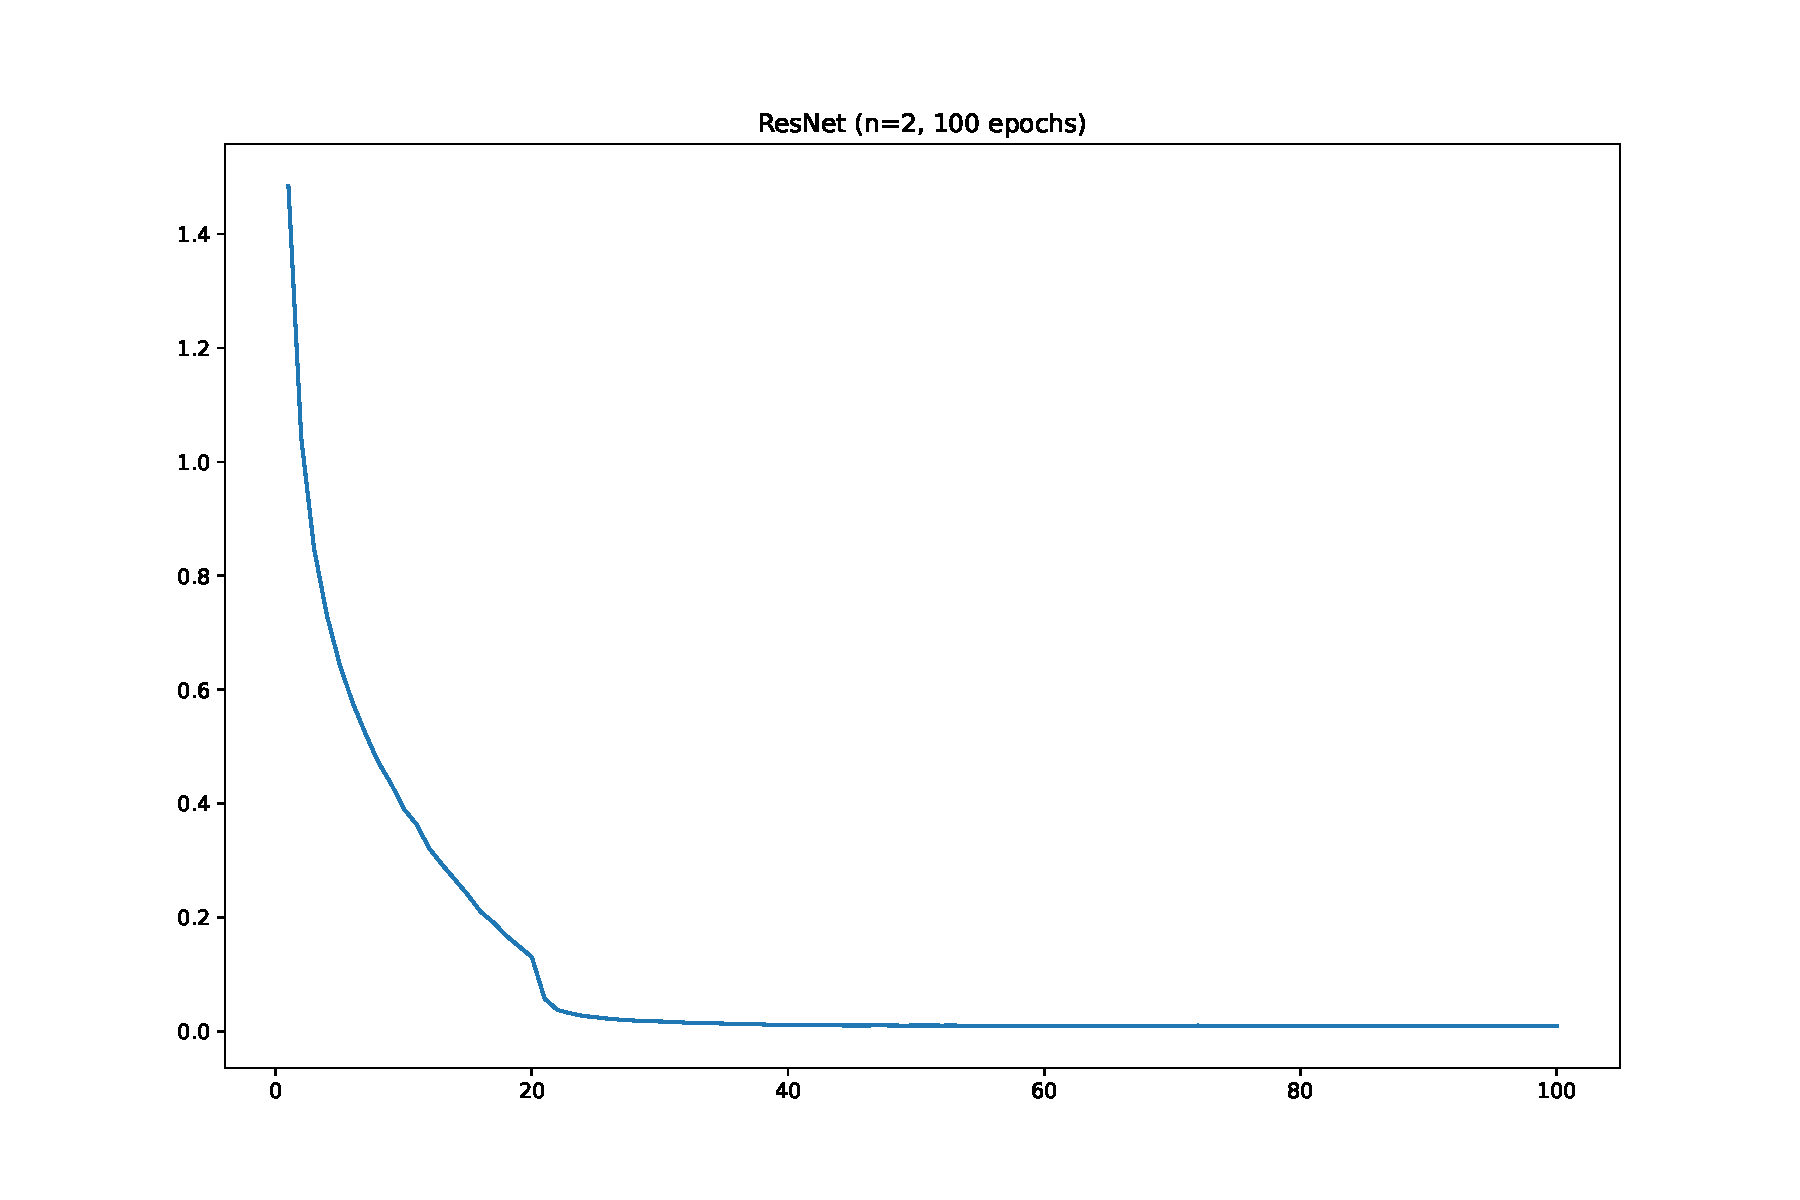
\includegraphics[width=0.7\textwidth]{../ResNet/q1_part2.pdf}
\end{figure}

\begin{figure}[!htbp]
\centering
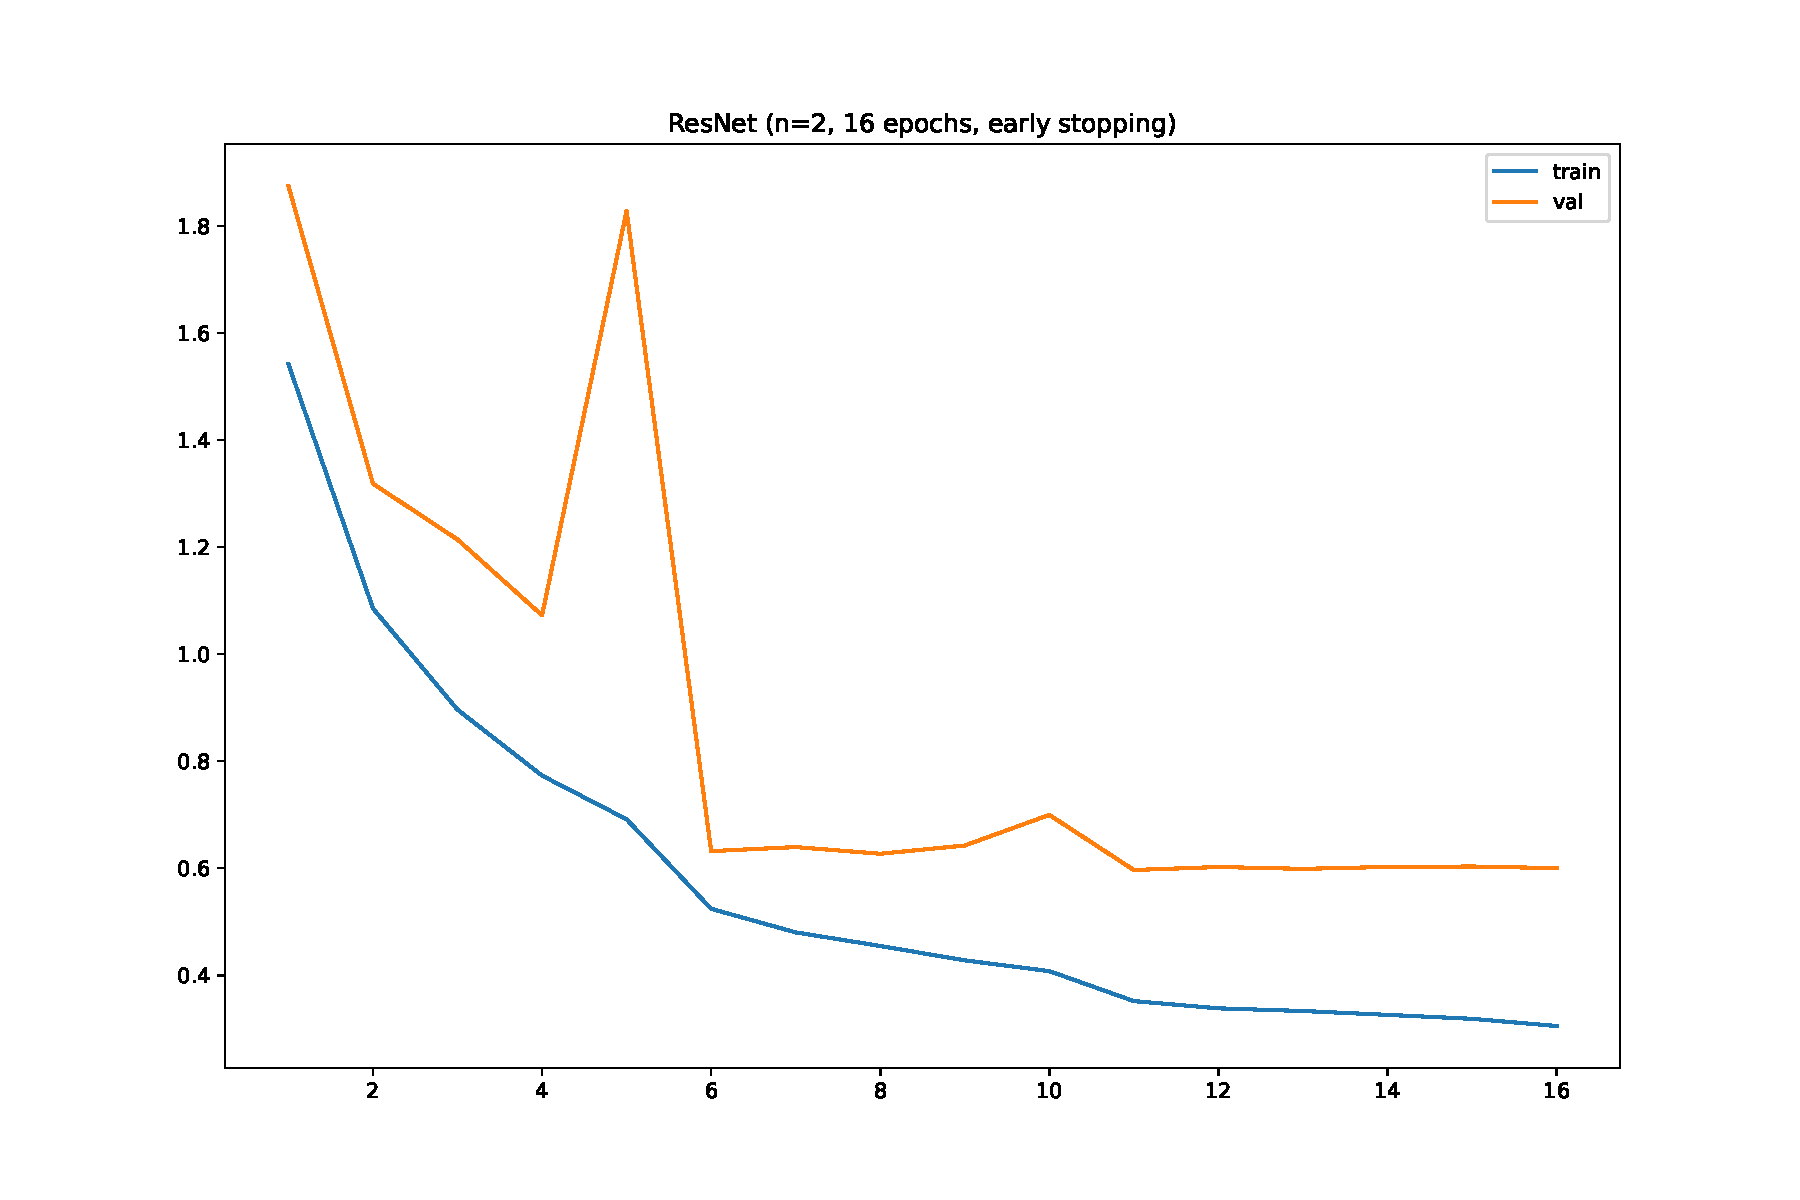
\includegraphics[width=0.7\textwidth]{../ResNet/q1_part3.pdf}
\end{figure}

\begin{center}
\begin{tabular}{|l|c|c|c|}
    \hline
    & Accuracy & F1 micro & F1 macro \\ 
    \hline
    train & 0.916 & 0.916 & 0.916 \\
    train & 0.797 & 0.797 & 0.796 \\
    train & 0.791 & 0.791 & 0.790 \\
    \hline
\end{tabular}
\end{center}

\subsection{Impact of Normalization}

\section{Text to SQL}


\end{document}
